\documentclass[10pt]{article}

\def\Type{LessonCaelan}
\def\TypeNum{Lesson 15}
\def\TypeTitle{Net Change, Area \& Definite Integrals }
\def\Semester{Fall 2021} %Not Used 
\def\Course{MATH 1190 \& 1210}
\def\Targets{  {\bf\color{Fuchsia}I1} }

\usepackage{preambleDJ}



%%%%%%%%%%%% BEGIN DOCUMENT %%%%%%%%%%%%%%%
%%%%%%%%%%%% BEGIN DOCUMENT %%%%%%%%%%%%%%%
%%%%%%%%%%%% BEGIN DOCUMENT %%%%%%%%%%%%%%%
%%%%%%%%%%%% BEGIN DOCUMENT %%%%%%%%%%%%%%%
%%%%%%%%%%%% BEGIN DOCUMENT %%%%%%%%%%%%%%%



\begin{document}

\pagestyle{otherpages}
\thispagestyle{firstpage}
\vs{.5}

\textbf{Intended Learning Outcomes}
After this lesson, you will be able to 

\itemC{
    \item Estimate definite integrals using rectangles of equal width. (\target{I1})
    \item Explain the meaning of a definite integral of a function in context, including determining the units of the integral. (\target{I1})
    \item Write mathematical expressions involving definite integrals to represent a given scenario. (\target{I1})
}

\vspace{-0.25cm}

\hrulefill\\

\vs{-.2}
During our first lesson of the semester, we asked ``how are slope, rate of change, and net change related?". So far, we've discovered that slope and AROC are identical in a linear relationship, and that the slope of a tangent line is identical to IROC. However, we have not meaningfully related net change to any of these quantities.\\

Now that we've extensively developed a tool $-$ the derivative $-$ that can measure slopes \& IROC, we can begin to make better sense of the relationship between these quantities and net change. In this lesson, we will begin by using IROC estimating net change, and then introduce a new tool that can measure net change directly.\\

{\example}\ltrm{\target{I1}} Similarly to the online pre-class assignment, $x(t)$ represents the position (in meters) of the object from the origin at time $t$ (in seconds).  The graph of the velocity $x^{\prime}(t)= v(t)$ (in m/sec) of an object is given below, where $t$ is the time (in sec) since the object's movements were initially measured. 
    \begin{enumerate}
    \item[(a)] Estimate the net change $\Delta x$ in the position of the object between $2$ and $4$ seconds after measurements were intially taken.  Recall that {\em Distance = Rate $\times$ Time} (if {\em Rate} is constant).
    \end{enumerate}
%
\vs{-.2}\hs{-.5}\mpageTth{.3}{.6}{.3}{\flushleft
%{ % Start a local group
  %\captionsetup{justification=raggedright, singlelinecheck=false}
\begin{minipage}{1.875in}
\centering
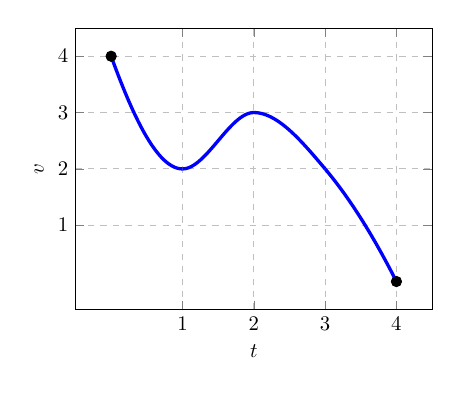
\begin{tikzpicture}[scale=0.75]
          \begin{axis}[
        %    axis y line = left,
        %    axis x line = bottom,
            xlabel = {$t$},
            ylabel = {$v$},
            xtick       = {1,2,3,4},
            xticklabels = {$1$,$2$,$3$,$4$},
            ytick       = {-2,-1,1,2,3,4,5,6},
            yticklabels = {$-2$,$-1$,$1$,$2$,$3$,$4$,$5$,$6$},
            samples     = 320,
            domain      = 0:4,
            %restrict y to domain=-5:5,
            xmin = -0.5, xmax = 4.5,
            ymin = -0.5, ymax = 4.5,
            width=3in,height=2.5in,
            grid=both, grid style=dashed
          ]
               \addplot[blue, ultra thick, mark=none, smooth, domain=0:1]  {4-7* x/2 + x^2 + x^3/2};
          \addplot[blue, ultra thick, mark=none, smooth, domain=1:2]  {7 - 12*x + 9*x^2 - 2*x^3};
          \addplot[blue, ultra thick, mark=none, smooth, domain=2:3]  {-7 + 12*x - 9/2* x^2 + x^3/2};
          \addplot[blue, ultra thick, mark=none, smooth, domain=3:4]  {2 + 3*x/2 - x^2/2};
         %
         \filldraw (0,4) circle (2.5pt);
         %
         \filldraw (4,0) circle (2.5pt);
         \end{axis}
    \end{tikzpicture}
       \vs{-.1} \captionof*{figure}{\bf \footnotesize{ Approach $\#1$:\\Left endpoints}}
       \end{minipage}
 %      }
}{
\mbox{}
}{\flushright
%{ % Start a local group
%  \captionsetup{justification=raggedleft, singlelinecheck=false}
\begin{minipage}{1.875in}
\centering
 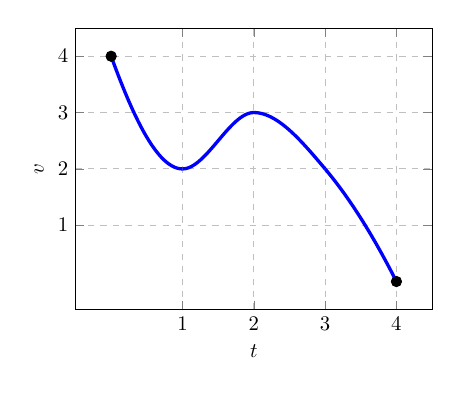
\begin{tikzpicture}[scale=0.75]
          \begin{axis}[
        %    axis y line = left,
        %    axis x line = bottom,
            xlabel = {$t$},
            ylabel = {$v$},
            xtick       = {1,2,3,4},
            xticklabels = {$1$,$2$,$3$,$4$},
            ytick       = {-2,-1,1,2,3,4,5,6},
            yticklabels = {$-2$,$-1$,$1$,$2$,$3$,$4$,$5$,$6$},
            samples     = 320,
            domain      = 0:4,
            %restrict y to domain=-5:5,
            xmin = -0.5, xmax = 4.5,
            ymin = -0.5, ymax = 4.5,
            width=3in,height=2.5in,
            grid=both, grid style=dashed
          ]
               \addplot[blue, ultra thick, mark=none, smooth, domain=0:1]  {4-7* x/2 + x^2 + x^3/2};
          \addplot[blue, ultra thick, mark=none, smooth, domain=1:2]  {7 - 12*x + 9*x^2 - 2*x^3};
          \addplot[blue, ultra thick, mark=none, smooth, domain=2:3]  {-7 + 12*x - 9/2* x^2 + x^3/2};
          \addplot[blue, ultra thick, mark=none, smooth, domain=3:4]  {2 + 3*x/2 - x^2/2};
         %
         \filldraw (0,4) circle (2.5pt);
         %
         \filldraw (4,0) circle (2.5pt);
         \end{axis}
    \end{tikzpicture}
       \vs{-.1} \captionof*{figure}{\bf \footnotesize{ Approach $\#2$:\\Right endpoints}}
       \end{minipage}
}
\vs{.2}~\\
\begin{enumerate}
\item[(b)] Given $t$ is assigned to the horizontal axis and $v$ is assigned to the vertical axis, how might we represent the quantity we computed in part (a) graphically? Sketch such a representation, and describe it in words below.
\end{enumerate}
\vs{-.2}\hs{-.5}\mpageT{.3}{.75}{
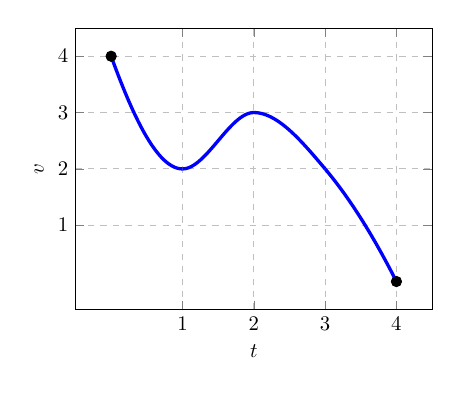
\begin{tikzpicture}[scale=0.75]
          \begin{axis}[
        %    axis y line = left,
        %    axis x line = bottom,
            xlabel = {$t$},
            ylabel = {$v$},
            xtick       = {1,2,3,4},
            xticklabels = {$1$,$2$,$3$,$4$},
            ytick       = {-2,-1,1,2,3,4,5,6},
            yticklabels = {$-2$,$-1$,$1$,$2$,$3$,$4$,$5$,$6$},
            samples     = 320,
            domain      = 0:4,
            %restrict y to domain=-5:5,
            xmin = -0.5, xmax = 4.5,
            ymin = -0.5, ymax = 4.5,
            width=3in,height=2.5in,
            grid=both, grid style=dashed
          ]
               \addplot[blue, ultra thick, mark=none, smooth, domain=0:1]  {4-7* x/2 + x^2 + x^3/2};
          \addplot[blue, ultra thick, mark=none, smooth, domain=1:2]  {7 - 12*x + 9*x^2 - 2*x^3};
          \addplot[blue, ultra thick, mark=none, smooth, domain=2:3]  {-7 + 12*x - 9/2* x^2 + x^3/2};
          \addplot[blue, ultra thick, mark=none, smooth, domain=3:4]  {2 + 3*x/2 - x^2/2};
         %
         \filldraw (0,4) circle (2.5pt);
         %
         \filldraw (4,0) circle (2.5pt);
         \end{axis}
    \end{tikzpicture}
}{
\mbox{}
}
\begin{enumerate}
\item[(c)] $x(t)$ represents the position of the object from the origin at time $t$.  Based on your answer in part (a), if the object was at position $10$ meters at $2$ seconds after measurements were initially taken, then approximately where is the object $4$ seconds after measurements were taken?



\end{enumerate}

%%%%%%%%%%%%%%%%%%%%%%%%%%%%%%%%%%%%%%%%%%%%%%%%%%%%%%%%%%%%%%%%%%%%%%%%%%%%%%%%%%%%%%%%%%%%%
\newpage%\end{document}%%%%%%%%%%%%%%%%%%%%%%%%%%%%%%%%%%%%%%%%%%%%%%%%%%%%%%%%%%%%%%%%%%%%%%%%%%%%%%%%%%%%
%%%%%%%%%%%%%%%%%%%%%%%%%%%%%%%%%%%%%%%%%%%%%%%%%%%%%%%%%%%%%%%%%%%%%%%%%%%%%%%%%%%%%%%%%%%%%

{\exercise}\ltrm{\bf\color{Fuchsia}I1} The weight, $w$ (in pounds), of a baby  is described by a function $w(t)$ where $t$ represents weeks after birth.  Below is a graph of the {\em growth rate} $w'(t)$ (in pounds per week) of an infant's weight $t$ weeks after birth. 
%
\begin{center}
    \begin{minipage}[t][2in][t]{0.275\textwidth}
    \,\\[-0.1in]
    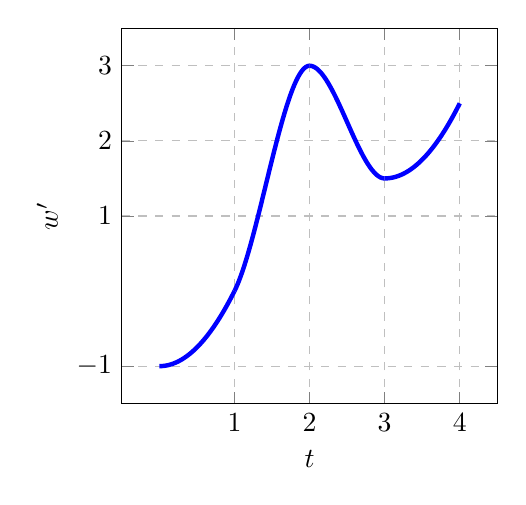
\begin{tikzpicture}
          \begin{axis}[
        %    axis y line = left,
        %    axis x line = bottom,
            xlabel = {$t$},
            ylabel = {$w'$},
            xtick       = {-2,-1,1,2,3,4,5,6},
            xticklabels = {$-2$,$-1$,$1$,$2$,$3$,$4$,$5$,$6$},
            ytick       = {-2,-1,1,2,3,4,5,6},
            yticklabels = {$-2$,$-1$,$1$,$2$,$3$,$4$,$5$,$6$},
            samples     = 320,
            domain      = -3:7,
            %restrict y to domain=-5:5,
            xmin = -0.5, xmax = 4.5,
            ymin = -1.5, ymax = 3.5,
            width=2.5in,height=2.5in,
            grid=both, grid style=dashed
          ]
         %
         % \addplot[blue, ultra thick, mark=none, smooth] coordinates{ (0,-1) (1,0) (2,3)  (3,1.5) (4,2.5)};
         %% In Mathematica, use ResourceFunction["CubicMonotonicInterpolation"][coords]. to find interpolating polynomial.
          \addplot[blue, ultra thick, mark=none, smooth, domain=0:1]  {x^2-1};
          \addplot[blue, ultra thick, mark=none, smooth, domain=1:2]  {7 - 20*x + 17*x^2 - 4* x^3};
          \addplot[blue, ultra thick, mark=none, smooth, domain=2:3]  {-39 + 54*x - 22.5*x^2 + 3* x^3};
          \addplot[blue, ultra thick, mark=none, smooth, domain=3:4]  {x^2-6*x+10.5};
         %
         \end{axis}
    \end{tikzpicture}
    \end{minipage}
    %
    \quad
    %
    \begin{minipage}[t][2in][t]{0.625\textwidth}
        \begin{enumerate}
        \item[(a)] Estimate the net change $\Delta w$ in the infant's weight from birth to $4$ weeks. Sketch rectangles whose areas represent your estimate. ({\it Note:} There are many correct answers to this prompt!)
        \end{enumerate}
    \end{minipage}
\end{center}
\vs{1}
\begin{enumerate}
\item[(b)] Based on your answer in part (a), if the infant weighed 7 pounds at birth, then approximately how much did the infant weigh when the infant was 4 weeks old?\\[0.5in]

\end{enumerate}
\vfill
{\bf\color{blue}Mini-lecture.} ({\it net change, area, and the definite integral})

\mpageTfour{.25}{.25}{.25}{.35}{
    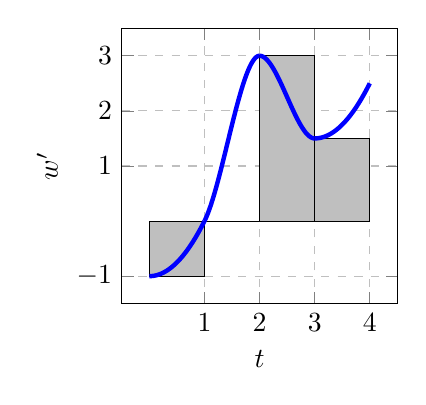
\begin{tikzpicture}
          \begin{axis}[
        %    axis y line = left,
        %    axis x line = bottom,
            xlabel = {$t$},
            ylabel = {$w'$},
            xtick       = {-2,-1,1,2,3,4,5,6},
            xticklabels = {$-2$,$-1$,$1$,$2$,$3$,$4$,$5$,$6$},
            ytick       = {-2,-1,1,2,3,4,5,6},
            yticklabels = {$-2$,$-1$,$1$,$2$,$3$,$4$,$5$,$6$},
            samples     = 320,
            domain      = -3:7,
            %restrict y to domain=-5:5,
            xmin = -0.5, xmax = 4.5,
            ymin = -1.5, ymax = 3.5,
            width=2in,height=2in,
            grid=both, grid style=dashed
          ]
         %
            \draw [fill=lightgray]  (3,1.5) rectangle (4,0); 
         \draw [fill=lightgray]  (2,3) rectangle (3,0); 
            \draw [fill=lightgray] (1,0) rectangle (2,0); 
            \draw [fill=lightgray] (0,-1) rectangle (1,0.0); 
         % \addplot[blue, ultra thick, mark=none, smooth] coordinates{ (0,-1) (1,0) (2,3)  (3,1.5) (4,2.5)};
         %% In Mathematica, use ResourceFunction["CubicMonotonicInterpolation"][coords]. to find interpolating polynomial.
          \addplot[blue, ultra thick, mark=none, smooth, domain=0:1]  {x^2-1};
          \addplot[blue, ultra thick, mark=none, smooth, domain=1:2]  {7 - 20*x + 17*x^2 - 4* x^3};
          \addplot[blue, ultra thick, mark=none, smooth, domain=2:3]  {-39 + 54*x - 22.5*x^2 + 3* x^3};
          \addplot[blue, ultra thick, mark=none, smooth, domain=3:4]  {x^2-6*x+10.5};
         %
         \end{axis}
    \end{tikzpicture}
    }{
    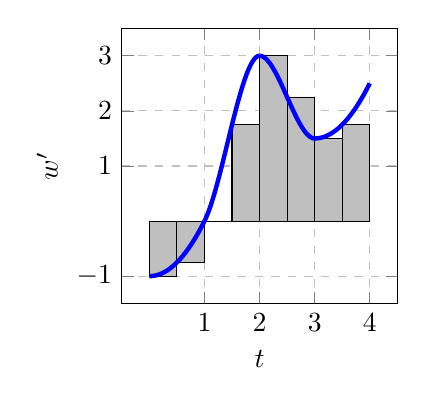
\begin{tikzpicture}
          \begin{axis}[
        %    axis y line = left,
        %    axis x line = bottom,
            xlabel = {$t$},
            ylabel = {$w'$},
            xtick       = {-2,-1,1,2,3,4,5,6},
            xticklabels = {$-2$,$-1$,$1$,$2$,$3$,$4$,$5$,$6$},
            ytick       = {-2,-1,1,2,3,4,5,6},
            yticklabels = {$-2$,$-1$,$1$,$2$,$3$,$4$,$5$,$6$},
            samples     = 320,
            domain      = -3:7,
            %restrict y to domain=-5:5,
            xmin = -0.5, xmax = 4.5,
            ymin = -1.5, ymax = 3.5,
            width=2in,height=2in,
            grid=both, grid style=dashed
          ]
         %
         \draw [fill=lightgray] (3.5,1.75) rectangle (4,0);
            \draw [fill=lightgray]  (3,1.5) rectangle (3.5,0); 
            \draw [fill=lightgray] (2.5,2.25) rectangle (3,0);
         \draw [fill=lightgray]  (2,3) rectangle (2.5,0); 
         \draw [fill=lightgray] (1.5,1.75) rectangle (2,0);
            \draw [fill=lightgray] (1,0) rectangle (1.5,0); 
            \draw [fill=lightgray] (.5,-.75) rectangle (1,0);
            \draw [fill=lightgray] (0,-1) rectangle (.5,0); 
         % \addplot[blue, ultra thick, mark=none, smooth] coordinates{ (0,-1) (1,0) (2,3)  (3,1.5) (4,2.5)};
         %% In Mathematica, use ResourceFunction["CubicMonotonicInterpolation"][coords]. to find interpolating polynomial.
          \addplot[blue, ultra thick, mark=none, smooth, domain=0:1]  {x^2-1};
          \addplot[blue, ultra thick, mark=none, smooth, domain=1:2]  {7 - 20*x + 17*x^2 - 4* x^3};
          \addplot[blue, ultra thick, mark=none, smooth, domain=2:3]  {-39 + 54*x - 22.5*x^2 + 3* x^3};
          \addplot[blue, ultra thick, mark=none, smooth, domain=3:4]  {x^2-6*x+10.5};
         %
         \end{axis}
    \end{tikzpicture}
    }{
        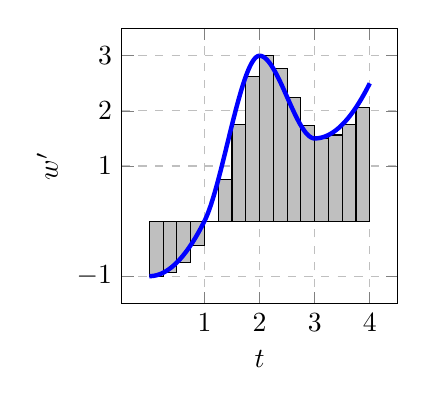
\begin{tikzpicture}
          \begin{axis}[
        %    axis y line = left,
        %    axis x line = bottom,
            xlabel = {$t$},
            ylabel = {$w'$},
            xtick       = {-2,-1,1,2,3,4,5,6},
            xticklabels = {$-2$,$-1$,$1$,$2$,$3$,$4$,$5$,$6$},
            ytick       = {-2,-1,1,2,3,4,5,6},
            yticklabels = {$-2$,$-1$,$1$,$2$,$3$,$4$,$5$,$6$},
            samples     = 320,
            domain      = -3:7,
            %restrict y to domain=-5:5,
            xmin = -0.5, xmax = 4.5,
            ymin = -1.5, ymax = 3.5,
            width=2in,height=2in,
            grid=both, grid style=dashed
          ]
         %
           \draw [fill=lightgray] (3.75,2.0625 ) rectangle (4,0);
         \draw [fill=lightgray] (3.5,1.75) rectangle (3.75,0);
           \draw [fill=lightgray] (3.25,1.5625 ) rectangle (3.5,0);
            \draw [fill=lightgray]  (3,1.5) rectangle (3.25,0); 
              \draw [fill=lightgray] (2.75,1.73438 ) rectangle (3,0);
            \draw [fill=lightgray] (2.5,2.25) rectangle (2.75,0);
              \draw [fill=lightgray] (2.25,2.76563 ) rectangle (2.5,0);
         \draw [fill=lightgray]  (2,3) rectangle (2.25,0); 
           \draw [fill=lightgray] ( 1.75,2.625) rectangle (2,0);
         \draw [fill=lightgray] (1.5,1.75) rectangle (1.75,0);
           \draw [fill=lightgray] ( 1.25,.75) rectangle (1.5,0);
            \draw [fill=lightgray] (1,0) rectangle (1.25,0); 
              \draw [fill=lightgray] ( .75,-.4375) rectangle (1,0);
            \draw [fill=lightgray] (.5,-.75) rectangle (.75,0);
             \draw [fill=lightgray] ( .25,-.9375) rectangle (.5,0);
            \draw [fill=lightgray] (0,-1) rectangle (.25,0); 
         % \addplot[blue, ultra thick, mark=none, smooth] coordinates{ (0,-1) (1,0) (2,3)  (3,1.5) (4,2.5)};
         %% In Mathematica, use ResourceFunction["CubicMonotonicInterpolation"][coords]. to find interpolating polynomial.
          \addplot[blue, ultra thick, mark=none, smooth, domain=0:1]  {x^2-1};
          \addplot[blue, ultra thick, mark=none, smooth, domain=1:2]  {7 - 20*x + 17*x^2 - 4* x^3};
          \addplot[blue, ultra thick, mark=none, smooth, domain=2:3]  {-39 + 54*x - 22.5*x^2 + 3* x^3};
          \addplot[blue, ultra thick, mark=none, smooth, domain=3:4]  {x^2-6*x+10.5};
         %
         \end{axis}
    \end{tikzpicture}
    }{
    \begin{flushright}
            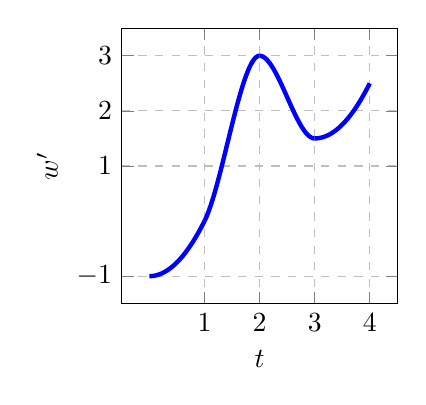
\begin{tikzpicture}
          \begin{axis}[
        %    axis y line = left,
        %    axis x line = bottom,
            xlabel = {$t$},
            ylabel = {$w'$},
            xtick       = {-2,-1,1,2,3,4,5,6},
            xticklabels = {$-2$,$-1$,$1$,$2$,$3$,$4$,$5$,$6$},
            ytick       = {-2,-1,1,2,3,4,5,6},
            yticklabels = {$-2$,$-1$,$1$,$2$,$3$,$4$,$5$,$6$},
            samples     = 320,
            domain      = -3:7,
            %restrict y to domain=-5:5,
            xmin = -0.5, xmax = 4.5,
            ymin = -1.5, ymax = 3.5,
            width=2in,height=2in,
            grid=both, grid style=dashed
          ]
         %
         % \addplot[blue, ultra thick, mark=none, smooth] coordinates{ (0,-1) (1,0) (2,3)  (3,1.5) (4,2.5)};
         %% In Mathematica, use ResourceFunction["CubicMonotonicInterpolation"][coords]. to find interpolating polynomial.
          \addplot[blue, ultra thick, mark=none, smooth, domain=0:1]  {x^2-1};
          \addplot[blue, ultra thick, mark=none, smooth, domain=1:2]  {7 - 20*x + 17*x^2 - 4* x^3};
          \addplot[blue, ultra thick, mark=none, smooth, domain=2:3]  {-39 + 54*x - 22.5*x^2 + 3* x^3};
          \addplot[blue, ultra thick, mark=none, smooth, domain=3:4]  {x^2-6*x+10.5};
         %
         \end{axis}
    \end{tikzpicture}
    \end{flushright}
    }
\vs{.5}
\newpage
\important{The Definite Integral}
{
Let $a$ and $b$ be real numbers with $a<b$, and suppose $f$ is continuous on the interval $[a,b]$. The {\bf definite integral} of $f$ from $a$ to $b$ is denoted by \[\int_a^b f(x)\,dx\] and represents the \unline{1}{}{.25} between the graph of $f$ and the interval along the $x$-axis from $a$ to $b$. If $f$ represents the rate of change of a quantity, then $\ds \int_a^b f(x)\,dx$ represents the \unline{1.5}{}{.25} in the quantity as $x$ varies from $a$ to $b$.
}
\example Based on the definition of definite integral, write down a mathematical expression representing the net change $\Delta w$ in the infant's weight from birth to 4 weeks for the scenario in Exercise A, and indicate its units.
\vs{.5}\\
\exercise\ltrm{\bf\color{Fuchsia}I1} Let $T'(t)$ represent the (instantaneous) rate of change (in $^{\circ}$C/day) of temperature in Charlottesville at a time $t$ (in days) during a particular week. 

\begin{enumerate}
\item[(a)] What are the units of $\ds \int_{1/2}^{3/2} T'(t)\,dt$? \vs{.2}

\item[(b)] What does this integral represent in the given context?
    \vfill

%\hfill ({\small\it continued on next page})

%%%%%%%%
%%%%%%%%%
%%%%%%%%%%
%%%%%%%%%%%
%\newpage%%%
%%%%%%%%%%%
%%%%%%%%%%
%%%%%%%%%
%%%%%%%%

\item[(c)] \pe If the temperature at noon on the first day of the week is $20^{\circ}$ C, then which of the following integral expressions represents the temperature at noon on the second day of the week?
   \enumAA{
        \item $20+\ds \int_{1/2}^{3/2} T'(t)\,dt$
        \item $20-\ds \int_{1/2}^{3/2} T'(t)\,dt$
        \item $\ds \int_{1/2}^{3/2} T'(t)\,dt-20$
        \item $\ds \int_{0}^{3/2} T'(t)\,dt$
        \item None of these options.
   }
\end{enumerate}

\newpage
{\exercise}\ltrm{\bf\color{Fuchsia}I1} The population of a country changes over time as people immigrate and emigrate. Suppose $f(t)$ gives the rate of change of the population $t$ years after officials began keeping records, in thousands per year. The graph of $f$ is given below.\\

\begin{minipage}[t]{0.3\textwidth}
\,\\[-0.1in]
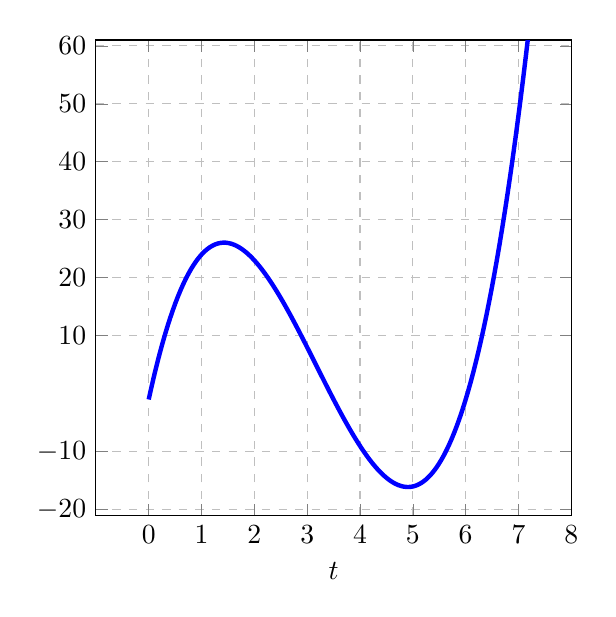
\begin{tikzpicture}
  \begin{axis}[
%    axis y line = left,
%    axis x line = bottom,
    xlabel = {$t$},
    %ylabel = { },
    xtick       = {0,1,2,3,4,5,6,7,8},
    xticklabels = {$0$,$1$,$2$,$3$,$4$,$5$,$6$,$7$,$8$},
    ytick       = {-20,-10,10,20,30,40,50,60},
    %yticklabels = {},
    samples     = 160,
    domain      = -1:3,
    restrict y to domain=-20:100,
    xmin = -1, xmax = 8,
    ymin = -21, ymax = 61,
    width = 3in, height=3in,
    grid=both, grid style=dashed
  ]
  \addplot[domain=0:8, blue, ultra thick] {-1+42*x-19*x^2+2*x^3};
\end{axis}
\end{tikzpicture}
\end{minipage}
%
\hfill
%
\begin{minipage}[t]{0.6\textwidth}
\begin{enumerate}
\item[(a)] Interpret in words the meaning of each of the following in terms of the context described above, including units.
    \begin{enumerate}
    \item[i.] $f(1)=24$\\[1.2in]

    \item[ii.] $\ds \int_1^7 f(t)\,dt$\\[0.8in]
    \end{enumerate}
\end{enumerate}
\end{minipage}

\begin{enumerate}
\item[(b)] Use 3 rectangles to estimate $\ds \int_1^7 f(t)\,dt$. Sketch rectangles whose areas represent your estimate. Note: There are many reasonable ways to do this!\\
\mpageT{.7}{.3}{
\,%%Room for solution later
}{
%%%Start2here
   \begin{flushright}
   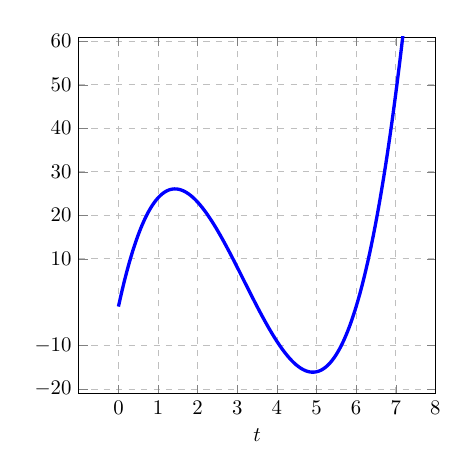
\begin{tikzpicture}[scale=.75]
  \begin{axis}[
%    axis y line = left,
%    axis x line = bottom,
    xlabel = {$t$},
    %ylabel = { },
    xtick       = {0,1,2,3,4,5,6,7,8},
    xticklabels = {$0$,$1$,$2$,$3$,$4$,$5$,$6$,$7$,$8$},
    ytick       = {-20,-10,10,20,30,40,50,60},
    %yticklabels = {},
    samples     = 160,
    domain      = -1:3,
    restrict y to domain=-20:100,
    xmin = -1, xmax = 8,
    ymin = -21, ymax = 61,
    width = 3in, height=3in,
    grid=both, grid style=dashed
  ]
  \addplot[domain=0:8, blue, ultra thick] {-1+42*x-19*x^2+2*x^3};
%    	\filldraw[red] (0,-1) circle (2.5pt);
%	\addplot[red, ultra thick, mark=none, smooth, domain=0:1]  {-1};
%      	\filldraw[red] (1,0) circle (2.5pt);
%	\addplot[red, ultra thick, mark=none, smooth, domain=1:2]  {0};
%      	\filldraw[red] (2,3) circle (2.5pt);
%	\addplot[red, ultra thick, mark=none, smooth, domain=2:3]  {3};
%	\filldraw[red] (3,1.5) circle (2.5pt);
%	\addplot[red, ultra thick, mark=none, smooth, domain=3:4]  {1.5};
%	\draw [fill=red, opacity=0.2]  (0,-1) rectangle (1,0); 
%	\draw [fill=red, opacity=0.2]  (2,3) rectangle (3,0); 
%	\draw [fill=red, opacity=0.2]  (3,1.5) rectangle (4,0); 
\end{axis}
\end{tikzpicture}
\end{flushright} 
}
\vs{1}
\item[(c)] Suppose the population $1$ year after officials began keeping records was $2000$. Write $-$ but do not solve $-$ an integral expression representing the number of people at time $t=4$.\\[0.5in]

\end{enumerate}


%%%%%%%%
%%%%%%%%%
%%%%%%%%%%
%%%%%%%%%%%
\newpage%%%
%%%%%%%%%%%
%%%%%%%%%%
%%%%%%%%%
%%%%%%%%


{\bf\color{blue}Extra Practice 1.}\ltrm{\bf\color{Fuchsia}I1} A faucet is pouring water into a tank, which happens to have a small hole in the bottom. Suppose $r(t)$ is the rate at which the volume of water in the tank is changing, measured in gallons per hour, $t$ hours after the faucet is turned on.
    \begin{enumerate}
    \item[(a)] Interpret in words the meaning of each of the following in the given context, including units.
        \begin{enumerate}
        \item[i.] $r(2)=-1$
            \vfill
        \item[ii.] $\ds \int_1^3 r(t)\,dt$
            \vfill
        \end{enumerate}

    \item[(b)] Write a mathematical expression representing the following.
        \begin{enumerate}
        \item[i.] the net change (in gallons) in the amount of water in the bucket two hours after the faucet is turned on
            \vfill

        \item[ii.] the initial rate (in gallons per hour) at which the volume of water in the tank is changing   
            \vfill
        \end{enumerate}

    \item[(c)] Suppose the tank initially contains $1$ gallon of water. Write an integral expression representing the amount of water in the bucket $2$ hours after the faucet is turned on.
        \vfill
    \end{enumerate}

\end{document}
